\documentclass{article}
\usepackage{cite}
\usepackage{amsmath,amssymb,amsfonts}
\usepackage{algorithmic}
\usepackage{graphicx}
\usepackage{textcomp}
\usepackage{xcolor}
\usepackage{hyperref}
\def\BibTeX{{\rm B\kern-.05em{\sc i\kern-.025em b}\kern-.08em
    T\kern-.1667em\lower.7ex\hbox{E}\kern-.125emX}}
\usepackage{graphicx} % Required for inserting images

\title{ML Final Project: Predicting Drug-Induced Autoimmune Responses}
\author{Anthony Clark}
\date{April 2025}

\begin{document}

\maketitle

\section{Introduction}

Drug-induced autoimmune responses can cause life-threatening and financially ruinous complications for drug design organizations when entering clinical trials. If a new drug causes a severe autoimmune response during clinical trials, this can be extremely hazardous to patients in the trials. Furthermore, the drug in question legally must be redesigned and may potentially be abandoned entirely. The ability to accurately predict whether or not a new drug will cause an autoimmune response when administered to human beings before clinical trials can save an enormous amount of money and protect the well-being of patients used in trials. When drugs are being developed in infancy, the primary biochemical mechanisms that guide decisions pertain to the specific target receptor or substrate. These mechanisms often ignore ancillary reactions that drugs can potentially cause in seemingly unrelated regions. For instance, a drug being designed to treat anxiety, might interact with receptors in the gut causing nausea or a drug being designed to treat skin dryness might interact with a receptor in the lungs causing congestion. The most immediately threatening receptors to consider when designing drugs are immune system receptors. Immune system receptors have evolved to combat and remove potentially harmful agents from the body. If immune receptors interact strongly with a potential drug, the drug is treated as an external threat by the body and the cascading immune response can be fatal. In preparation for combating potential drug-induced autoimmune responses, drug design organizations develop predictive models using physiochemical features such as "number of valence electrons", "binding affinity to {known} ligand", "number of hydroxyl groups", etc. as predictive variables to predict whether or not a particular drug will cause an autoimmune response during clinical trials, in humans. These physiochemcial features are often identical to the features used to predict whether or not a drug will interact favorably with a particular target receptor and so drug design organizations have access to data pertaining to these physiochemical features. 

Since immune systems are highly variable between patients, different patients will exhibit different degrees of autoimmune responses to different drugs. That being said, there is enough conservation and similarity among the general population for models to still possess predictive power. If a drug does not exhibit an autoimmune response during clinical trials, it will most likely not cause an autoimmune response in a vast majority of the population.%cite 

Due to recent developments in biochemical spectroscopy and measurement methods, physiochemical datasets can be relatively high-dimensional. To integrate these high-dimensional physiochemical datasets with classifiers, the datasets are often processed by dimensionality reduction and feature selection algorithms. In combination with dimensionality reduction, ensemble methods have shown to be extremely accurate when applied to physiochemical-based, drug-induced autoimmune response datasets.

In this project, I constructed and evaluated several classification pipelines to predict whether or not a certain molecule physiochemical profile will induce an autoimmune response in patients during clinical trials. The predictive power of these pipelines is evaluated by a combination of accuracy and recall score. 

\section{Dataset}

\subsection{Strengths and Weaknesses}

The dataset used in this project is from the UC Irvine Machine Learning Respository and was denoted on January 5th, 2025. I chose this dataset because it is relatively recent and the description claims that it is intended for ensemble learning classifiers. The dataset has 597 instances and 195 features, including the target variable. 

Each instance is a different drug, with a unique drug identifier, and each feature is a physiochemical measurement. These features include a wide array of measurements from number of valence electrons to binding affinities with particular ligands. The target variable in this dataset is binary and it denotes whether or not a particular drug has caused an autoimmune response in patients. 

This being a relatively high p : n ratio, I thought this dataset would be good for feature selection and dimensionality reduction techniques. The dataset has a lot of correlation between features, suggesting that they could be combined or selected out. 


\subsection{Biases}

The data is unbalanced with the number of positive cases making up about 25 percent of the drugs. This means that only 25 percent of the drugs in the dataset exhibited a drug-induced autoimmune response, meaning if a classifier simply always guessed that a drug does not cause a drug-induced autoimmune response, then it would be correct 75 percent of the time. 

There is a degree of sampling bias, the drugs presented in the dataset are drugs that have a wide range of measured physiochemical characteristics. A lot of drugs do not have values pertaining to certain physiochemical characteristics and so they have been included from the dataset simply because they are not available. 

\subsection{Preprocessing}

The following preprecessing steps were applied:
\begin{itemize}
\item Features with several "NA" values were removed
\item Features with several "Missing" or "Null" values were removed
\item Log values with -infinity were removed 
\item Three copies were created; standardized, normalized and log. Comparison between shown in results section
\item The original data was split between "train" and "test", the two files werer concatenated and then re-split depending on the train/test split ratio. 
\end{itimize}

\begin{figure}[hbt!]
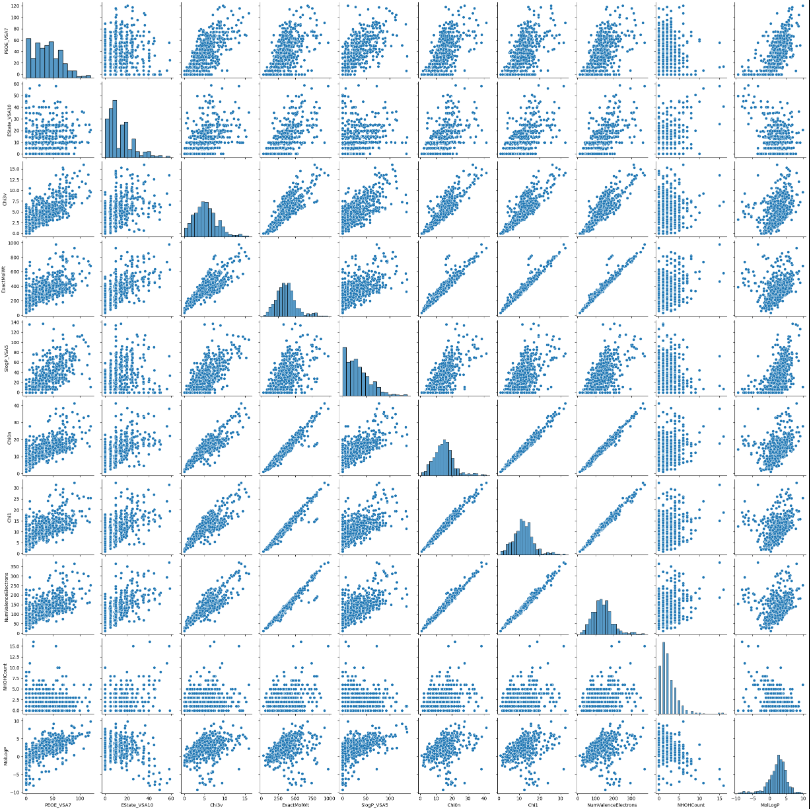
\includegraphics[width=8cm]{pairplot.PNG}
\caption{10 by 10 pairplot of 10 random features taken from the unscaled feature dataset}
\end{figure}

A number of pairplots were generated to look at the correlation between features. Strong linear relationships were observed across the entire unscaled dataset. Some relationships were so strong that one of the features was removed with the rationale being that the features are expressing the exact same information. 

\begin{figure}[hbt!]
\includegraphics[width=8cm]{01_REAL_001_ML_Final_cols18 to 28.png}
\caption{Histogram of 10 random features in the unscaled dataset}
\end{figure}

Histograms were generated for each of the 197 features in the unscaled dataset to visualize the distributions and skews. Skew values were also generated for each feature in the unscaled dataset to inform certain downstream transformations. Several features had the same value for every single entry, those features were removed from the unscaled dataset before any classifiers were applied. 

\section{Baseline Performance}

Before any feature selection or dimensionality reduction was applied, four different SVM kernels were applied:\newline
1) Linear\newline
2) Polynomial\newline
3) RBF\newline
4) Sigmoid\newline

The resulting confusion matrices are shown below:

\begin{figure}[hbt!]
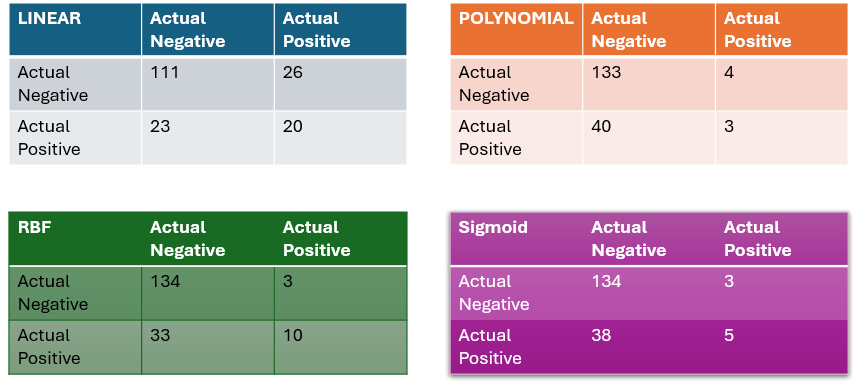
\includegraphics[width=8cm]{Baseline_accuracy_svm.PNG}
\caption{Confusion matrices for the four svm kernels in the baseline accuracy.}
\end{figure}


Because drug-induced autoimmune response is primarily concerned with false negatives, recall score is favored over total accuracy.\newline


Keep in mind that because of the 75/25 split of the 0/1 binary target variable, a model that only chooses 0 will be correct 75 percent of the time.\newline

Below are the accuracy and recall scores for each of the four svm kernels:
\begin{figure}[hbt!]
\includegraphics[width=5cm]{accuracy_metrics.PNG}
\caption{Accuracy and recall scores for the four svm kernels in the baseline accuracy.}
\end{figure} \newline

Although the linear kernel had the lowest accuracy, it had the highest recall score by two-fold when compared to the next highest recall score, corresponding to the rbf kernel.

A random forest was also trained at baseline. Some hyperparaamter tuning was done to maximize accuracy. Some further tuning was done to balance accuracy and recall scores. Figure 3 shows the parameters for the best random forest model before feature selection. 

\begin{figure}[hbt!]
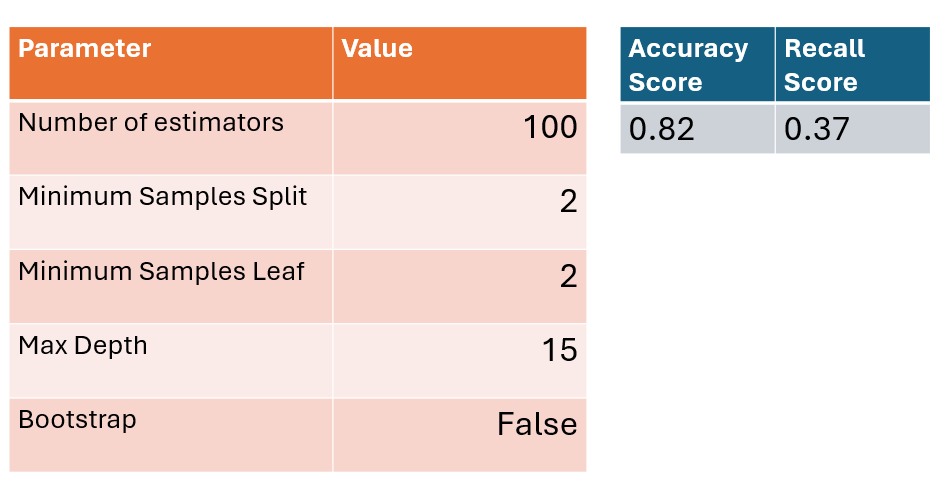
\includegraphics[width=8cm]{Baseline_random_forest.PNG}
\caption{Baseline random forest parameters with accuracy score and recall score}
\end{figure}

This baseline random forest was used to obtain feature importances for each of the features. Because there were 194 features, the names have been excluded from the x-axis. Figure 4 shows the feature importance. I decided to make a subset of the dataframe, using only features with feature importances above the 0.01 threshold. 

\begin{figure}[hbt!]
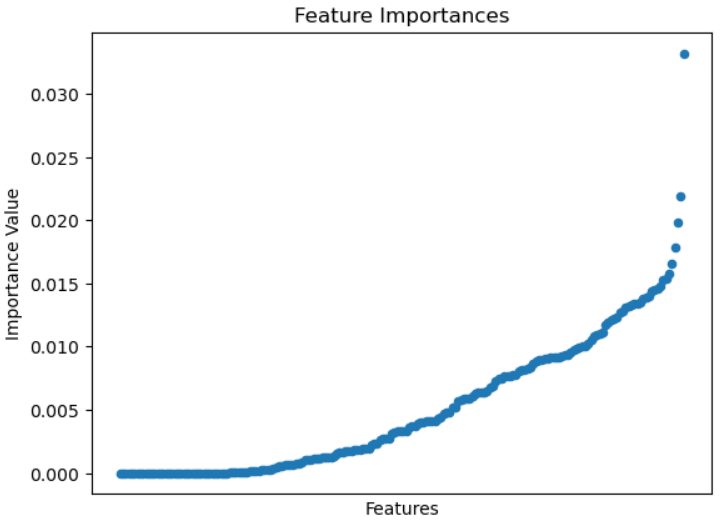
\includegraphics[width=8cm]{Feature Importances.PNG}
\caption{Feature Importances based on the tuned random forest model. Feature names have been excluded for visualization}
\end{figure}

First, the random forests model was tuned using random search. After hyperparameter tuning, the feature importances were plotted and a subset of features was selected based on the magnitude of feature importance. These features were also cross-checked with the loadings of the first principal components in the preliminary PCA analysis, however, an emphasis was placed on random forest feature importance since the first principal component only accounted for 5 percent of the cumulative explained variance. There was significant overlap between feature importance and principal component feature loadings, some of the same variables were within the top 10 features such as "Number of Valence Electrons" and the "Chi" linkage coefficients. These features were applied to four classifiers used in baseline; 1) random forests 2) logistic regression, 3) XGBoost, and 4) linear SVM. All of the recall scores using both the top 10 features and top 50 features in accordance to the random forests feature importance list yielded lower or equal recall scores in all four classifiers. 

\section{Experiments}

\subsection{Scaling Features}

I compared the accuracy scores and recall scores of four different models (random forests, logistic regression, XGBoost, LDA)  using three different scaling techniques (standardization, normalization, and logarithmic transform). The four models underwent hyperparameter tuning and the logarithmic transform was only applied to certain features, depending on the skew and spread. 



\begin{figure}[hbt!]
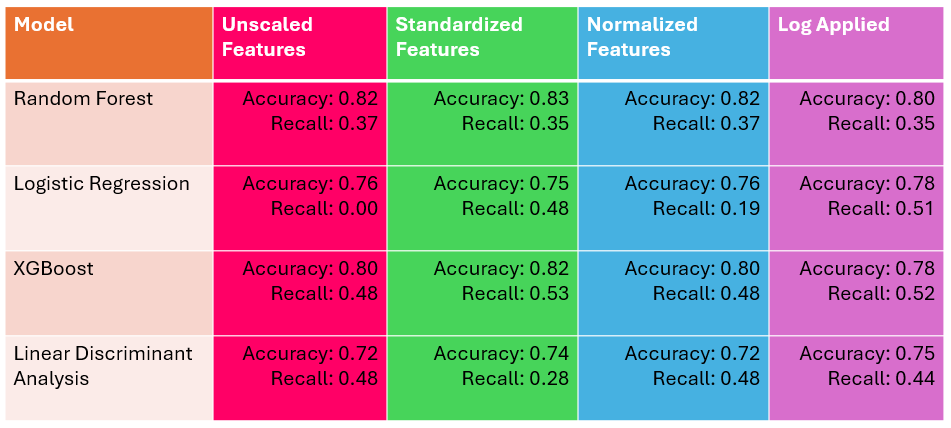
\includegraphics[width=8cm]{scaling.PNG}
\caption{The accuracy and recall scores for tuned random forests, logistic regression, XGBoost and linear discriminant analysis after different scaled data.}
\end{figure}

Different models respond differently to certain scaling techniques. Random forests was relatively unaffected by standardization, normalization and log transformations, whereas logistic regression was highly receptive to these three scaling techniques. The unscaled recall score for logistic regression was 0, but this increased to 0.53 when the features were standardized and 0.52 when the features underwent certain logarithmic transformations. Both linear discriminant analysis and XGBoost had a relatively high recall score when applied to the unscaled features. XGBoost saw a significant increase in recall, to 0.53 when applied to the standardized features whereas LDA saw a significant drop in recall score from 0.48 to 0.28. None of the scaling improved the LDA recall score, both the standardization and log transformation features saw lower recall scores with LDA. 

\subsection{Adding Features}

The first 50 features according to the sorted feature importance provided by the tuned random forest model, in the baseline evaluation, were selected, and polynomial transformations were applied to certain features, depending on their distributions and relationship with the target variable. Interaction columns were made for three combinations of variables:\newline \newline
1. "ExactMolWt" vs "Chi3v" \newline
2. "Chi0n" vs "Chi1" \newline
3. "NumValenceElectrons" vs "Chi1" \newline

All of these features are measurements of electron distributions thorough the biomolecule. The value of one will inevitably interact with the value of another. These interactions were used in addition to the original features in the classifiers. 

Lastly, two new features were derived; one a combinatorial "Chi" feature that adds all of the chi values and two a chi/mole ratio that takes the combination chi value and divides it by the exact molecular weight. Chi values measure the degree of linkage between atoms pertaining to a particular molecule, but chi values do not always take into account the weight of the atoms themselves. The chi/mole ratio takes the biomolecule's exact molecular weight into account. \newline

Figure 6 shows the accuracy and recall scores for the three types of added features (polynomial, interaction, and derived) with respect to the four tuned classifiers (random forests, logistic regression, XGBoost and LDA). 



\begin{figure}[hbt!]
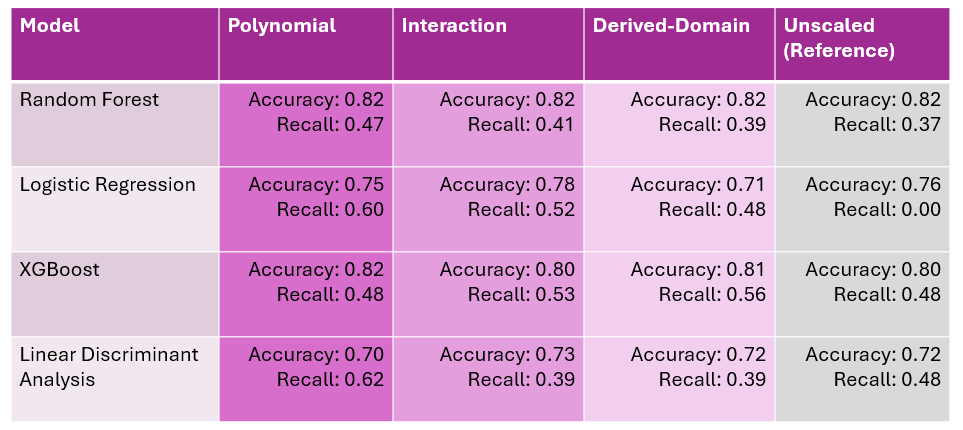
\includegraphics[width=8cm]{Adding_Features.PNG}
\caption{Shows the three different feature adding techniques (polynomial, interactions, and domain-specific derived features) and the corresponding accuracy and recall score for each of the four classifiers.}
\end{figure}


The polynomial transformations significantly improved the recall scores in both the logistic regression and linear discriminant analysis, with logistic regression improving by over 10 percent. The interactions decreased the recall score for the random forests, logistic regression and the linear discriminant analaysis. That being said, it did improve the recall score for the xgboost model. The domain-derived features yielded the best xgboost recall score out of the three feature additions at 0.56. The other three models saw a decrease in recall score when the domain-derived features were incorporated. 


\subsection{Feature Transformations}

Because linear discriminant analysis is one of the four classifiers used to evaluate the earlier experiments and the number of discriminants is limited to the number of classes in the target variable minus one, LDA was excluded from the feature transformation and PCA was applied instead. In binary classification, such as in the case of drug-induced autoimmune response, the number of classes is two and so the maximum amount of discriminants in LDA is equal to one. This is very limiting for hyperparameter tuning. That being said, the maximum number of components in a principal component analysis is equal to the minimum between the number of features and the number of samples, giving much more room for tuning. \newline

Four classifiers were used to evaluate the effect of principal component numbers of the accuracy and recall scores:\newline
1. Random Forests \newline
2. Logistic Regression \newline
3. Xgboost \newline
4. Support Vector Machine (linear kernel) \newline

The linear kernel was chosen for SVM because it had the largest recall score when comparing linear vs rbf vs polynomial vs sigmoid. \newline

A preliminary principal component analysis was run to see how many components are required to obtain a cumulative explained variance of around 90 percent. It was about 50 principal components, indicating that the feature data has a more complex structure and cannot simply be represented by a few linear combinations of the original variables. This indicates that the variables have a lot of inter-correlation and it takes multiple components to capture the underlying correlational interplay.
\begin{figure}[hbt!]
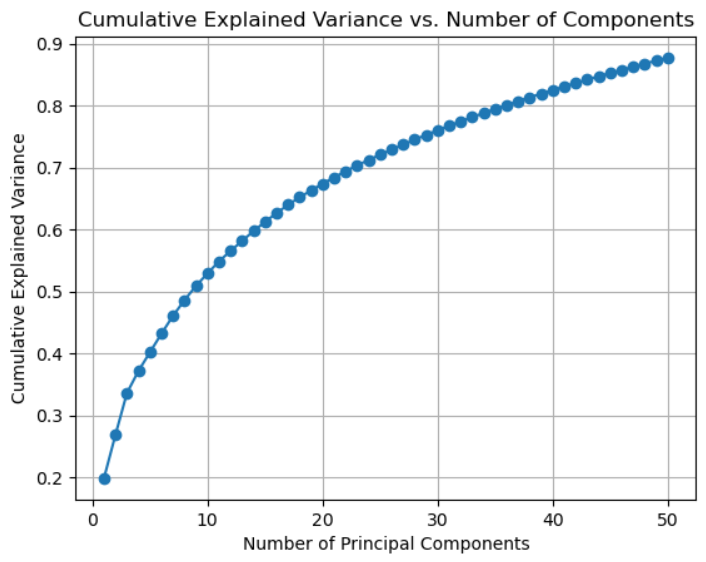
\includegraphics[width=8cm]{Cumulative Exaplained Variance.PNG}
\caption{Shows the Recall Score for the four classifiers 1) Random Forests 2) Logistic Regression 3) XGBoost 4) SVM *linear with respect to the number of principal components.}
\end{figure}

Hyperparameter tuning for the number of principal components in the linear PCA transformation prior to integration with the four classifiers 1) random forests 2) logistic regression 3) XGBoost and 4) SVM were performed and shown in the figure below. \newline

\begin{figure}[hbt!]
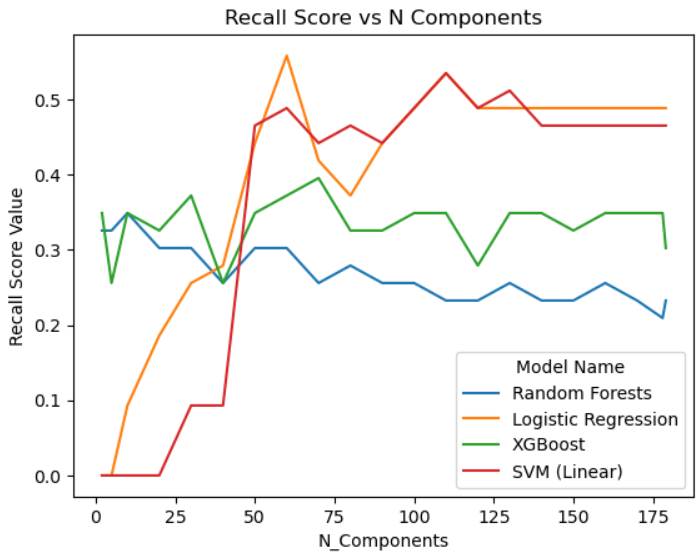
\includegraphics[width=8cm]{001_lineplot.PNG}
\caption{Shows the Recall Score for the four classifiers 1) Random Forests 2) Logistic Regression 3) XGBoost 4) SVM *linear with respect to the number of principal components.}
\end{figure}
\newline
\newline
The random forests recall score remained relatively unchanged as n components increased, in fact, the recall score was higher with lower n components whereas XGBoost slightly increased with n components. The logistic regression model saw a sharp increase in recall score as n components increased, peaking around 60 principal components and then subsequently plateauing around 110 principal components. SVM had a recall score of zero even with as much as 20 principal components, with a sudden jump around 25 principal components and again at around 50 principal components, also plateauing around 110 principal components. The highest recall score was logistic regression at around 0.62.\newline


\begin{figure}[hbt!]
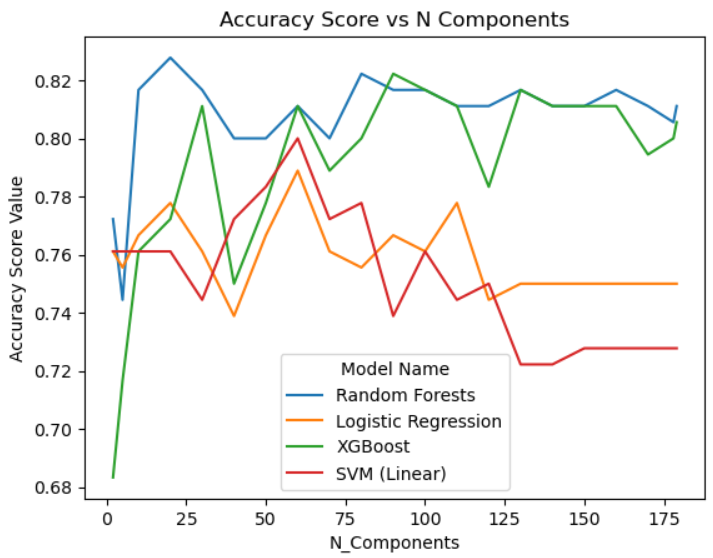
\includegraphics[width=8cm]{001_lineplot acc.PNG}
\caption{Shows the accuracy score for each of the four classifiers with respect to number of principal components in dimensionality reduction.}
\end{figure}
\newline
\newline

When comparing the two graphs between accuracy scores and recall scores vs number of principal components, there is a clear trade off between the two evaluation metrics. As logistic regression recall score increases with number of principal components, the corresponding accuracy score starts to decrease. 

\subsection{Noisy Indicators}

Random variables were added to the normalized dataset so that the values could be strictly defined as between 0 and 1, within the same domain as the other features. After adding each random variable, accuracy and recall scores were calculated for each of the following four classifiers; 1) Random Forests, 2) Logistic Regression, 3) XGBoost, 4) SVM kernel = linear. The addition of random variables caused slight fluctuations in the  accuracy scores and recall scores of the four classifiers, but remained relatively unchanged. XGBoost.



\begin{figure}[hbt!]
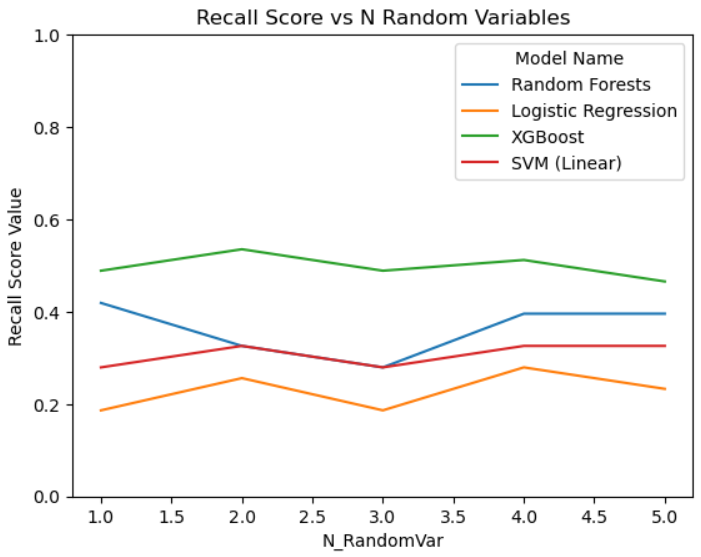
\includegraphics[width=8cm]{Random_recall.PNG}
\caption{Shows the recall scores for the four classifiers with respect to number of random variables added to the dataset.}
\end{figure}

XGBoost exhibited the least amount of fluctuations as the number of random variables were added to the dataset, suggesting it may be the most resilient to noise introduction of the four classifiers, when measuring recall score. 

\begin{figure}[hbt!]
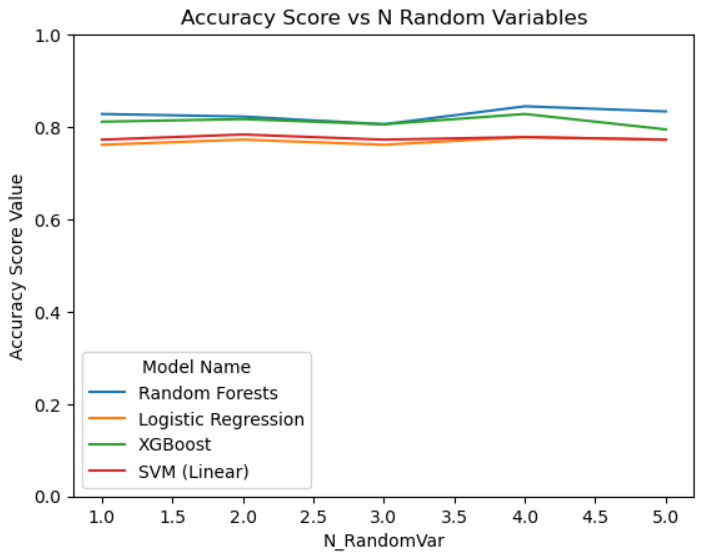
\includegraphics[width=8cm]{accuracy_random.PNG}
\caption{Shows the accuracy scores for the four classifiers with respect to number of random variables added to the dataset.}
\end{figure}

Although XGBoost was the most resilient to random noise when measuring recall score, the linear kernel support vector machine exhibited the least number of fluctuations, of the four classifiers, when measuring accuracy score. This is evidence of how different classifiers exhibit varying degrees of resilience to noise, depending on the evaluation metric. 

\subsection{Interpretation}

SHAP interaction summary plots were used to selection the "top 10" interactive features, although the resulting accuracy and recall scores declined heavily. It appears that the underlying dataset is too complex and cannot be reduced to 10 features. 

\begin{figure}[hbt!]
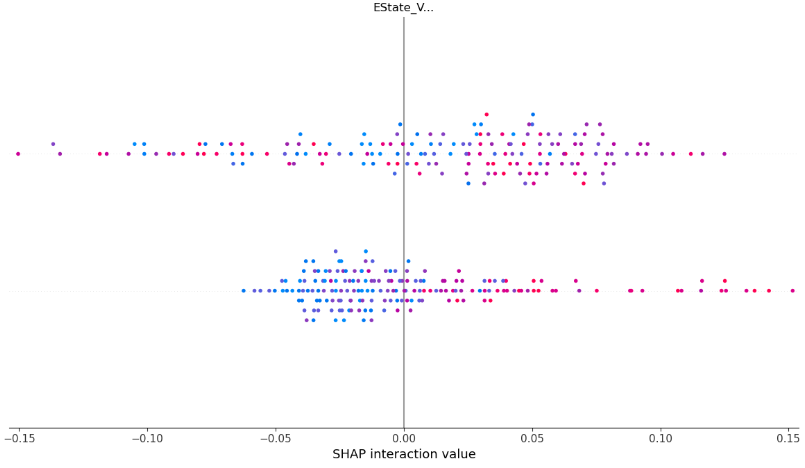
\includegraphics[width=8cm]{SHAP.PNG}
\caption{Example of one of the interaction plots, close up on the variable EState_VSA10 or "electron state VSA10", one of the most interactive variables.}
\end{figure}

Due to the underlying complexity of the dataset as represented by the initial PCA-based cumulative explained variance chart, a simple SHAP interaction plot will not be enough for feature selection. Interpretability relies heavily on a combination of domain-knowledge and more complex modeling.  


\subsection{Training Times}

The model efficiency for four classifiers; 1) random forests 2) logistic regression 3) XGBoost and 4) linear SVM were measured with respect to number of principal components used to transform the feature dataset. 

\begin{figure}[hbt!]
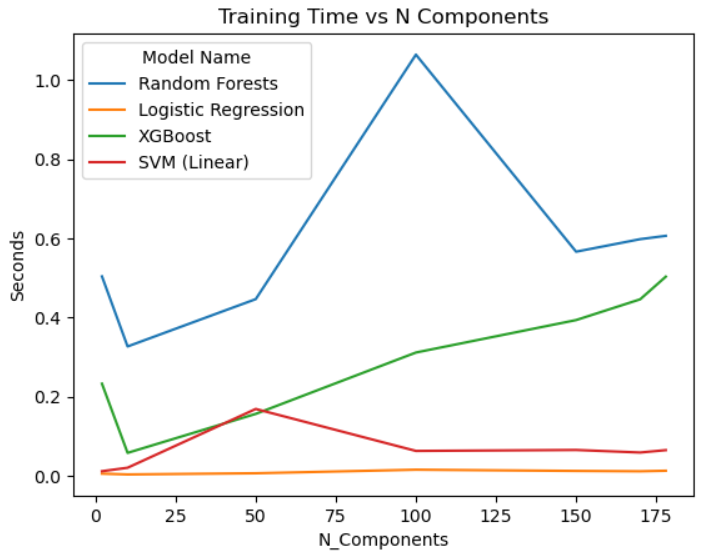
\includegraphics[width=8cm]{0Training_time_vs_n_components.PNG}
\caption{Shows the training time of the four classifiers with respect to number of principal components used to transform the feature dataset.}
\end{figure}

Both training time and inference time have a non-linear relationship with number of principal components used to transform the feature dataset. Both see a significant decline time as n components is increased and there does seem to be some trade-offs between training and prediction time. Training time for XGBoost seems to have a partial linear relationship with n components after n components = 10. Random forests saw a massive spike in training time between n components = 50 and n components = 100. This is surprising because random forests is a parallelizable model, where XGboost is less so. The spike in training time for random forests is consistent with the inference time spike also seen around the same n components values for random forests. It seems that the number of principal components may have more complicated effects on the underlying model efficiency. Logistic regression consistently had very low training times and inference times when compared to the other three classifiers. Linear SVM had relatively stable training and inference times with a slight spike in training time around n components = 50, with a subsequent drop around n components = 60 and a plateau around n components = 100. 



\begin{figure}[hbt!]
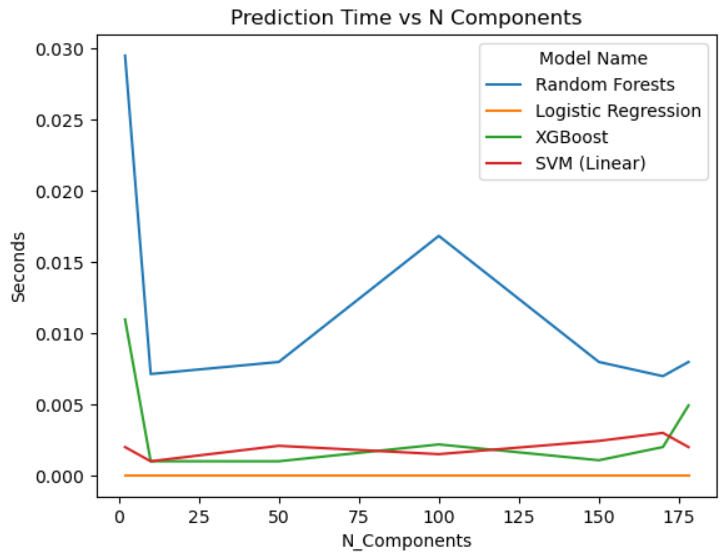
\includegraphics[width=8cm]{01Prediction_time_vs_n_components.PNG}
\caption{Shows the inference time of the four classifiers with respect to number of principal components used to transform the feature dataset.}
\end{figure}

Random forests had consistently higher training times and inference times when compared to the other three classifiers across all of the number of principal components. Conversely, logistic regression consistently had the smalleset training and inference times when compared to the other three classifiers across all principal components. 

\section{Recommend Model}

The objective of model tuning is to maximize recall, which takes into account false negatives, the most costly error types in clinical trials, while also maintaining an accuracy score above the baseline of 0.75. There is inevitably a tradeoff between accuracy and recall score, although there are approached/pipelines that increase both with respect to baseline. After examining all of the approaches used in this project, the approaches that yielded the highest recall scores while also improving accuracy were logistic regression paired with polynomial transformations, logistic regression paired with PCA number of components equal to 60. That being said, logistic regression consistently yielded the lowest recall scores using unscaled and other transformations. The selective logarithmic transform also yielded relatively high recall scores in logistic reggresion as well as XGBoost. XGBoost show a significantly high recall score when using the combined interaction features and domain-specific derived feature such as "Chi" combination. The preliminary cumulative explained variance plot is consistent with the logistic regression recall score improvement. As the number of principal components approaches 60, which is approximately when 95 percent of cumulative exlained variance is reached, the corresponding recall scores for the logistic regression model is optmized, around 0.65. The linear SVM recall scores also show exhibit this behavior with slightly lower recall scores with respect to logistic regression. It is important to note that as the number of principal components is increased, both logistic regression and linear SVM show a sharp decline in recall score, with a subsequent recovery around n components = 100. The recall scores for Random forests actually declined with respect to number of principal components, although remaining relatively stable. Interestingly enough, the accuracy score for random forests saw a decline between n components = 2 and n components = 5 with a massive spike at n components = 20, then subsequent plataeu. XGBoost also exhibited a massive spike between n components = 2 and n components = 20 in accuracy, with the recall score being moderatively consistent across all principal component numbers. \newline

With all the aforementioned responses considered, logistic regression paired with the n components = 60 PCA transformed feature data had the highest recall scores with an accuracy at 0.80, baseline accuracy of 0.75. Logistic regression paired with polynomial and selected-logarithmically transformed feature datasets, exhibited the second highest recall scores, also with accuracy metrics above baseline. Logistic regression without these vital transformations will yield extremely low recall scores and baseline accuracy scores. \newline

XGBoost and linear discriminant analysis show consistently high recall score with the domain-specific and interaction combination feature dataset paired with XGBoost yielded a recall score of 0.61 and an accuracy score of 0.82. Linear discriminant analysis yielded 0.50 recall scores and 0.80 accuracy scores without any prior transformation.\newline

If transformations are possible and domain specific knowledge can be applied then logistic regression paired with certain transformations yield the highest cumulative recall and accuracy scores with PCA of n components = 60 having the highest recall score. Linear SVM also yielded consistently high recall and accuracy scores with PCA n components = 60 having a high recall score and above baseline accuracy score. If analysis time is limited and transformations are not possible, then XGBoost and linear discriminant analysis yielded the highest recall and accuracy scores with unscaled, untransformed features. \newline

Random forests consistently yielded low recall scores when compared to the other classifiers when applied to transformed feature datasets. This is especially true when looking at PCA transformations, random forests consistently yielded lower recall scores across almost all of the number of principal components. Random forests accuracy scores, in constrast remain relatively high, but due to the nature of the dataset and the problem of drug-induced autoimmune responses, accuracy score alone is not enough to evaluate the performance of a classifier. 

\section{Future Work}

\subsection{Non-linear PCA}
Linear PCA transformations exhibited significant increases in recall scores when paired with certain classifiers, it would be interesting to see the impact on recall when applied non-linear, kernel PCA transformations. Large amounts of non-linear relationships were observed during pairwise analysis. Due to the relatively high volume of features, all of the pairwise combinations could not be thoroughly evaluated. The scope of this project was primarily constrained to observing linear relationships. That being said, a combination of linear and non-linear transformations may be able to yield more favorable recall and accuracy metrics. The PCA cumulative variance and random forests feature importance show a significant complex information amount features, but the some of the overwhelming relationships may in fact be non-linear. 

\subsection{Advanced Ensembles}

More advanced ensemble techniques, such as voting or utilizing a meta learner may in fact yield more favorable results. Considering that different classifiers exhibit higher recall scores depending on the feature data transformation, a meta learner or voting ensemble algorithm that combines the outputs of multiple classifiers could yield considerably higher recall scores. 

\subsection{Domain Knowledge}

Due to the inherent complexity of drug design and physiochemical structural measurements, a considerable amount of domain-knowledge can help undercover the underlying complexity in the dataset. With what limited domain-knowledge I possess, I was able to greatly improve the recall score of XGBoost combining the "Chi", molecular linkage coefficients. This was only a intimate knowledge of 3 of the 197 features. Considerable domain knowledge of all of the features is essentially to improving the recall score above 0.65. Even after considerable preprocessing, it's important to know what features are essentially describing the same underlying phenomenon, but with different scales. I was able to remove a few with what little domain knowledge I possess, but I imagine there are still several features that express the exact same physical molecular information, but in slightly different scales or representations.  

\end{document}
